\documentclass[10pt,a4paper]{article}
\usepackage{amsmath}
\usepackage{amsfonts}
\usepackage{amssymb}
\usepackage{graphicx}
\usepackage{lmodern}
\usepackage{enumerate}
\usepackage{subcaption}
\usepackage{hyperref}
\author{Bert Peters --- s1147919}
\title{Homework 3}
\begin{document}
\maketitle

\section{Spider}

Using the framework provided I created my web spider. For this, I added code to main, as well as improving the \texttt{GetNextURL} and \texttt{ShiftP} methods. Most importantly, I fixed \texttt{GetNextURL} so that the links it returns do not contain a newline. The final code runs quite well for multiple pages. For extracting data, I reused my implementation from last time.

When running the program, my program suddenly stopped after finding its first \texttt{null} response. The problem, it turned out, was that the LIACS Cups server did not respond properly to my request. I removed the exit statement on that line, and my program went on to query 57,000 links before its queue was full.

The program can be compiled by running \texttt{make} in either the root directory or the spider directory. It will produce some warnings, but those are all located in the htmlstreamparser library.

\section{Duplicate detection}

My program implements a simple form of duplicate detection. It adds links one by one, checking for each link whether it is already in there.

To check if a link is already in the queue, I do substring search using \texttt{strstr} for the new link followed by a newline. If this is not found, I append the new link to the queue.

The algorithm above is not the most efficient algorithm, as it needs to look up every string in the queue, which has complexity that is approximately linear in the size of the queue. A proper solution would be to have some smart index of crawled links, that would require for example a hashset.

When we are doing this, we might also implement a queue in a smarter way than a long newline separated string, for example with a queue of string pointers.

\section{Salient Point Detection}
\begin{enumerate}[a)]
	\item Looking at the pictures, I found that the algorithm find sharp edges in the pictures. It works quite well to find the edge of the Notre Dame in the first picture, because it has a huge contrast with the sky behind it. The windows are also nicely lined. because of this.

	\item Tom Cruise's face has about half the salient points as does the Notre Dame. This is easily explained: faces do not have as much hard edges as buildings. The matcher works quite well. It correctly matched the corners of both his eyes, a patch on his cheek and the tip of his nose. The RANSAC parser was actually worse: it removed a single correct connection whilst adding none.

	\item I took some pictures of the collected works of Sir Arthur Conan Doyle. In several varying angles, I ran the program the program and compared the matching point. Book 0 was the straight picture, and the angle increased with the numbers. The straight shot has 427 salient points. The matching points were as follows:
	\begin{center}
	\begin{tabular}{l|r|r|r}
	Book \# & Points & Matching & RANSAC\\
	\hline
	1 & 320 & 158 & 147 \\
	2 & 353 & 113 & 104 \\
	3 & 358 & 79 & 71 \\
	4 & 393 & 45 & 30 \\
	5 & 584 & 20 & 19
	\end{tabular}
	\end{center}
	The reason for the additional points in the fifth picture is that there is now some additional furniture in the shot. The pictures can be seen in \autoref{fig:sherlock}. The matches between the programs are shown in \autoref{fig:matches}. The RANSAC algorithm does remove some invalid matches here.

	\item I wrote similarimage.cpp to accomplish this. The program takes exactly three arguments and will output the one that it considers the most similar to the first. Because my previous experiments showed mixed results on when using the RANSAC algorithm, I used the simple one.

	The program will compile using \texttt{make} in the sift directory, or when running it in the root directory. When run, it will look approximately like \autoref{fig:similarimage}.
\end{enumerate}

\begin{figure}
    \centering
    \begin{subfigure}[b]{0.3\textwidth}
        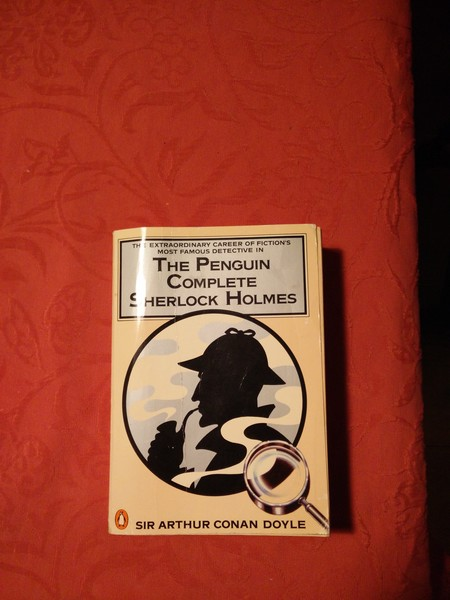
\includegraphics[width=\textwidth]{sift/books/0.jpg}
        \caption{Front picture}
    \end{subfigure}
    \begin{subfigure}[b]{0.3\textwidth}
        \includegraphics[width=\textwidth]{sift/books/0.jpg.sift.jpg}
        \caption{Salient points}
    \end{subfigure}
    \begin{subfigure}[b]{0.3\textwidth}
        \includegraphics[width=\textwidth]{sift/books/5.jpg.sift.jpg}
        \caption{Side picture}
    \end{subfigure}
    \caption{Pictures of Sherlock Holmes}
\label{fig:sherlock}
\end{figure}

\begin{figure}
	\centering
	\begin{subfigure}[b]{0.3\textwidth}
	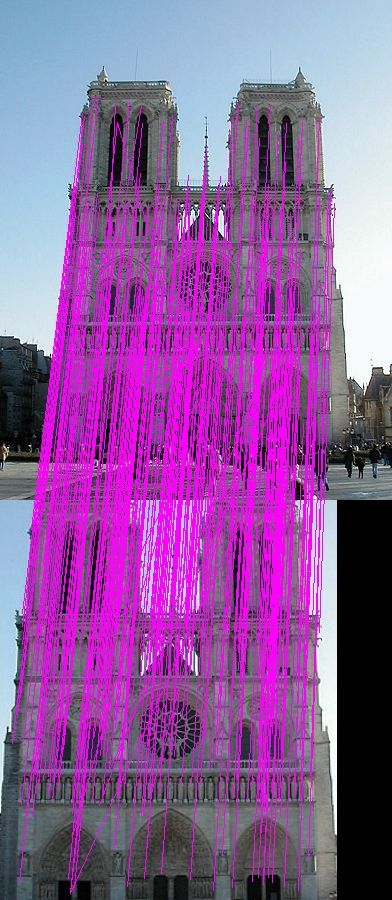
\includegraphics[width=\textwidth]{sift/matches}
	\caption{Regular matches}
	\end{subfigure}
	\begin{subfigure}[b]{0.3\textwidth}
	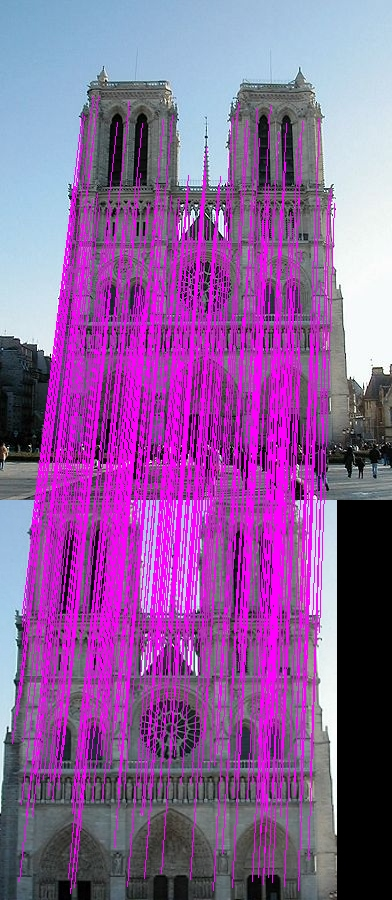
\includegraphics[width=\textwidth]{sift/matches.ransac.jpg}
	\caption{RANSAC matches}
	\end{subfigure}
	\caption{Matches between the different angles.}
	\label{fig:matches}
\end{figure}

\begin{figure}
	\centering
	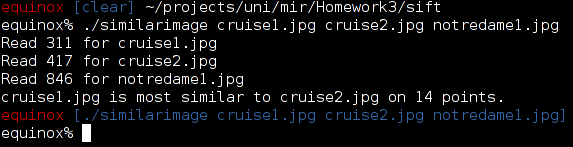
\includegraphics[width=\textwidth]{screenshot}
	\caption{The similarimage program in action.}
	\label{fig:similarimage}
\end{figure}
\end{document}
